\chapter{\scshape CVMix Parameterizations}
\label{chapter:cvmix_intro}

\minitoc
\vspace{.5cm}

We provide in this chapter an overview of the vertical mixing
parameterizations available with CVMix.


\section{Vertical mixing parameterizations in CVMix}
\label{section:vert_mix_schemes_cvmix}

The CVMix Project aims to address the needs of various ocean modeling
groups to code, test, tune, and document parameterizations of oceanic
vertical mixing for numerical ocean simulations.  Phase I of the
project has focused on first-order turbulence closures for vertical
mixing processes.  Future development may consider higher order
schemes, motivated by developments with the General Ocean Turbulence
Model (GOTM) from \cite{GOTM}.  Notably, CVMix does {\it not}
determine time stepping for the model prognostic fields.  Instead,
time stepping is the responsibility of the calling model code.  

The following schemes are included in the CVMix parameterizations
during Phase I of the development.
\begin{itemize}

\item {\sc Static background mixing} (Chapter
  \ref{chapter:cvmix_background}): Certain turbulent processes, in
  particular the ambient background gravity wave ``noise'', constitute
  a background level of mixing that is largely steady in time from the
  pespective of large-scaling ocean modeling.  Though assumed to be
  time independent, these processes generally have a nontrivial space
  dependence.  CVMix provides options for various of these time
  independent schemes:
\begin{itemize}
\item the vertical profile from \cite{BryanLewis1979};
% \item the profile from \cite{Henyey_etal1986} in which mixing near the
%   equator is very small, as measured by \cite{Gregg_etal2003}; 
% \item the approaches from \cite{Jochum2009}, in which enhanced mixing
%   from parametric subharmonic mixing is included. 
\end{itemize}


\item {\sc Shear induced mixing} (Chapter \ref{chapter:cvmix_shear}):
  The following schemes are available for shear mixing:
 \begin{itemize}
 \item \cite{PPvmix}, applicable largely for tropical circulation;
 \item \cite{LargeKPP} and \cite{Large_Gent1999}, which builds on the
   \cite{PPvmix} scheme;
  \end{itemize}


\item {\sc Tidally induced mixing} (Chapter
  \ref{chapter:cvmix_tidal}): The following schemes are available for
  parameterizing mixing induced by ocean tides.
  \begin{itemize}
   \item \cite{Simmonsetal2004} 
\end{itemize}


\item {\sc Double diffusive processes} (Chapter
  \ref{chapter:cvmix_ddiffusion}): Double diffusive processes arise
  from the distinct mixing properties of temperature relative to
  salinity and other material tracers.

\item {\sc KPP surface boundary layer} (Chapter
  \ref{chapter:cvmix_kpp}): The K-profile parameterization (KPP)
  scheme from \cite{LargeKPP} provides for a diffusivity as well as a
  non-local transport, each within the surface planetary boundary
  layer.

\item {\sc Vertical convective mixing}: Vertical profiles can become
  gravitationally unstable, such as when the ocean is forced with a
  negative buoyancy flux.  Older approaches such as \cite{CoxModel}
  and \cite{Rahmstorf1993} considered a convective {\it adjustment}
  algorithm, in which vertical pairs of grid cells were adjusted
  towards a profile of static stability.  In effect, the vertical
  diffusivity is infinite when using adjustment schemes.  CVMix does
  {\it not} provide options for convective adjustment.  Instead, CVMix
  allows for the specification of a diffusivity that is large in
  regions of gravitational instability, thus enabling vertical
  convective {\it mixing} rather than {\it adjustment}.  Notably, when
  using the KPP surface boundary layer scheme, convective mixing is
  {\it not} computed inside the KPP boundary layer.  Instead, it is
  only computed beneath the boundary layer, and it is done so {\it
    after} the KPP boundary layer matching has occurred (see Section
  \ref{section:vert_mix_schemes_ordering_cvmix}).


\end{itemize}


\section{General form of CVMix parameterizations}
\label{section:vert_mix_schemes_general_cvmix}

CVMix focuses only on vertical transport processes in the ocean, so
that we are concerned with the tracer or velocity equation in the form
\begin{equation}
  \frac{\partial \overline{\lambda} }{\partial t}  = 
 - \frac{\partial}{\partial z}  \left( \overline{w' \, \lambda'} + \overline{w} \, \overline{\lambda} \right). 
\end{equation}
In this equation, $w'$ is the turbulent or fluctuating portion of the
vertical velocity\footnote{In Chapter \ref{chapter:cvmix_kpp}, we
  follow the notation of \cite{LargeKPP} by writing the mean
  quantities with an uppercase, $W$ and $\Lambda$, and turbulent
  fluctuations with a lowercase, $w$ and $\lambda$. For the present
  chapter, we follow the more standard notation of equation
  (\ref{eq:mean-turbulent-decompose-w}).}
\begin{equation}
 w = w' + \overline{w},
\label{eq:mean-turbulent-decompose-w}
\end{equation}
$\lambda'$ is a fluctuating scalar or velocity component
\begin{equation}
 \lambda = \lambda' + \overline{\lambda},
\label{eq:mean-turbulent-decompose-lambda}
\end{equation}
and the overline denotes an Eulerian ensemble or time average that
separates the mean flow from turbulent fluctuations.  The vertical
flux $\overline{w} \, \overline{\lambda}$ is represented in a
numerical model by an advection operator or remapping operation, and
it is comprised of flow {\it resolved} by the model grid.  In
contrast, $\overline{w' \, \lambda'}$ is the correlation between
fluctuations in the vertical velocity component and the field
$\lambda$. This correlation is often termed the {\it turbulent flux}
of $\lambda$.  It is not explicitly represented by a numerical model,
since it arises from processes at the subgrid scale.  CVMix code
provides a suite of closures, or {\it parameterizations}, for this
subgrid scale flux.

We are interested in those correlations $\overline{w' \, \lambda'}$
that can be parameterized in terms of vertical diffusion or vertical
non-local mixing.  That is, all parameterizations considered in CVMix
can be formulated in terms of a diffusivity and a non-local transport,
in which case the turbulent flux is written as
\begin{equation}
  \overline{w' \, \lambda'} = 
  -K_{\lambda} \,  \left(  \frac{\partial \overline{\lambda}}{\partial z} \right)
 + K^{\mbox{\tiny non-local}}_{\lambda} \,  \gamma_{\lambda}.
\label{eq:cvmix-parameterization}
\end{equation}
The first term on the right hand side of equation
(\ref{eq:cvmix-parameterization}) provides for the familiar
downgradient vertical diffusion determined by a non-negative vertical
diffusivity, $K_{\lambda} \ge 0$, and the local vertical derivative of
the model's resolved field, $\partial \overline{\lambda} / \partial
z$.  This term is referred to as the local portion of the vertical
mixing parameterization
\begin{equation}
\overline{ w' \, \lambda' }^{\, \mbox{\scriptsize local}} = -K_{\lambda} \left( \frac{\partial \overline{\lambda}}{\partial z} \right).
\end{equation}
Note that the term ``local'' is used for this portion of the
parameterized flux (\ref{eq:cvmix-parameterization}) since it is
determined by the local derivative of the mean field,
$\overline{\lambda}$.  However, the diffusivity can generally be
determined as a non-local function of boundary layer properties, with
such being the case for the KPP scheme (Chapter
\ref{chapter:cvmix_kpp}).  

The second term in equation (\ref{eq:cvmix-parameterization}),
$\gamma_{\lambda}$, accounts for non-local transport that is not
directly associated with local vertical gradients of $\lambda$, in
which we have
\begin{equation}
\overline{w' \, \lambda'}^{\, \mbox{\scriptsize non-local}} = K^{\mbox{\tiny non-local}}_{\lambda}  \; \gamma_{\lambda}.
\label{eq:non-local-transport-intro}
\end{equation}
KPP is the only scheme available with CVMix that prescribes a nonzero
value for $\gamma_{\lambda}$.  In the original implementation from
\cite{LargeKPP}, they considered $K^{\mbox{\tiny non-local}}_{\lambda}
= K_{\lambda}$. However, as noted in Sections
\ref{section:vert_mix_schemes_ordering_cvmix} and
\ref{subsection:kpp-shape-function}, that prescription leads to
problems for the non-local flux $\overline{w' \, \lambda'}^{\,
  \mbox{\scriptsize non-local}}$ for those cases where the diffusivity
$K^{\mbox{\tiny non-local}}_{\lambda}$ at the base of the boundary
layer does not vanish.  When $K^{\mbox{\tiny non-local}}_{\lambda}$
does not vanish at the boundary layer base, then the non-local flux
has a spurious jump condition across the boundary layer base, since
the flux vanishes below the boundary layer. We leave further details
of this issue for the discussion in Section
\ref{subsection:kpp-shape-function}, where we argue that the KPP
scheme should set {\it both} its local and non-local fluxes smoothly
to zero at the boundary layer base.

Every scheme available in CVMix computes parameterized turbulent
fluxes based on a suite of inputs from the calling model, such as the
surface buoyancy and momentum fluxes, vertical stratification, and
vertical shear.  There may also need to be information about the
bottom roughness and unresolved tide speeds.  Besides the diffusivity
and non-local transport, various diagnostic fields are available to
help understand the internal workings of the parameterizations.



\section{KPP matching and ordering the CVMix schemes}
\label{section:vert_mix_schemes_ordering_cvmix}

Certain of the CVMix schemes represent parameterizations of processes
that are largely independent.  Their resulting diffusivities and
viscosities are thus added to produce a net mixing coefficient.  Other
schemes, however, must be called in a certain order given the
underlying assumptions built into the scheme.  The issue concerns the
KPP surface boundary layer scheme when used in a form according to
\cite{LargeKPP}, in which diffusivities are matched across the
boundary layer base.  We here summarize the two main issues associated
with this approach.
\begin{itemize}
\item {\sc KPP after interior non-convective mixing}: As implemented
  according to \cite{LargeKPP}, the KPP scheme matches diffusivities
  at the base of the boundary layer to values computed beneath the
  boundary layer (Section \ref{subsection:kpp-shape-function}).  In
  this case, KPP must be called subsequent to those schemes
  determining non-convective mixing coefficients in the ocean
  interior.  

\item {\sc KPP before interior convective mixing}: Again, if
  implementing KPP according to the methods from \cite{LargeKPP},
  diffusivity matching at the base of the KPP boundary layer
  intrinsically assumes there to be a transition from typically larger
  diffusivities in the boundary layer to typically smaller
  diffusivities in the interior.  However, this sort of transition
  cannot always be ensured, since gravitationally unstable water can
  appear beneath the boundary layer in which case the interior
  diffusivities can be quite large.  Problems with the diffusivity
  matching occur if insisting that KPP match its boundary layer
  diffusivity to a potentially large interior diffusivity arising from
  convective mixing.  These problems are ameliorated if parameterized
  convective mixing in the ocean interior is called {\it after} the
  KPP boundary layer scheme.  Furthermore, note that convective
  parameterizations are not used inside the KPP boundary layer, since
  KPP provides the mixing coefficients in the boundary layer.

\end{itemize}

The above concerns with the \cite{LargeKPP} implementation of KPP are
eliminated {\it if} one does not match the boundary layer diffusivity
to the interior diffusivity.  In this case, the KPP scheme and all
other schemes can be called in any order, with the resulting net
diffusivity used after all of the physical processes contribute to the
mixing coefficients.  This alternative simplified approach to the KPP
scheme is discussed in Section \ref{subsection:kpp-shape-function}.
We recommend using the simpler approach, unless aiming to reproduce
older results from KPP formulated using the \cite{LargeKPP} matching
conditions.

These considerations lead to the flow diagram shown in Figure
\ref{fig:vertical_mix_flow_cvmix} for use of CVMix schemes.

%%%%%%%%%%%%%%%%%%%% %%%%%%%%%%%%%%%%%%%%%%%%%
\begin{figure}[h!t]
\rule{\textwidth}{0.005in}
\begin{center}
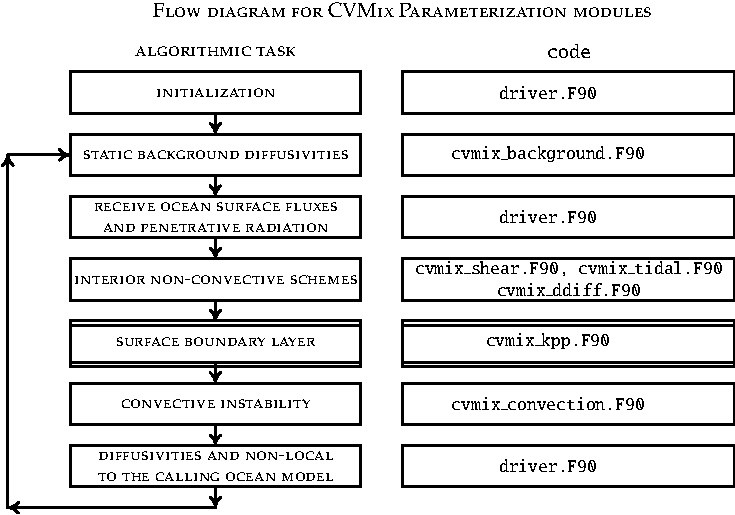
\includegraphics[angle=0,width=15cm]{./mfpic_figs/cvmix_flow_diagram.pdf}
\caption[Flow diagram for CVMix schemes]{\sf This flow diagram depicts
  the general algorithmic steps required to utilize the CVMix
  parameterization modules.  The initialization step occurs in the
  ocean model (e.g., MPAS-ocean, MOM, or POP) calling the CVMix
  modules.  This initialization serves to set up arrays and derived
  type structures, all as a function of the input that it receives
  from the calling ocean model code.  The next step during
  initialization is to call the module {\tt cvmix\_background.F90} to
  fill chosen static background diffusivities.  Upon entering the time
  dependent portion of the ocean model integration, the driver
  receives surface fluxes and penetrative radiative fluxes.  Calls are
  made to chosen interior non-convective mixing schemes, such as shear
  mixing, tide mixing, and double diffusion.  Thereafter, the surface
  boundary layer scheme is called, with KPP the scheme targetted for
  Phase I of CVMix.  If implementing the KPP scheme according to
  \cite{LargeKPP}, then the boundary layer calculation {\it must} come
  after the interior non-convective portion, and before the convective
  portion (see discussion in Section
  \ref{section:vert_mix_schemes_ordering_cvmix}).  If instead using
  the simpler approach detailed in Section
  \ref{subsection:kpp-shape-function}, then KPP can be called in any
  order within the calling tree.  After the boundary layer, then
  convective mixing is called, with regions of gravitationally
  unstable water given a large diffusivity.  Notably, if KPP is used
  for the surface boundary layer, parameterized convective mixing is
  generally performed only beneath the KPP boundary layer.  The final
  step returns the diffusivity $K_{\lambda}$, viscosity, and non-local
  transport $K^{\mbox{\tiny non-local}}_{\lambda} \; \gamma_{\lambda}$
  (equation (\ref{eq:non-local-transport-intro})), arrays to the
  calling ocean model code.  A new time step starts by reinitializing
  the diffusivities to their static background values.}
\label{fig:vertical_mix_flow_cvmix}
\end{center}
\rule{\textwidth}{0.005in}
\end{figure}
%%%%%%%%%%%%%%%%%%%%%%%%%%%%%%%%%%%%%%%%%%%%%%%%%%%%%%%%%%%%%%%%%%%%%%%%



